%%%%%%%%%%%%%%%%%%%%%%%%%%%%%%%%%%%%%%%%%%%%%%%%%%%%%%%%%%%%%%%%%%%%%%%%%%%%%%%%
%%%%%%%%%%%%%%%%%%%%%%%%%%%%%%%%%%%%%%%%%%%%%%%%%%%%%%%%%%%%%%%%%%%%%%%%%%%%%%%%
%\documentclass[addpoints,12pt,solution]{exam}
\documentclass[preprint,12pt]{elsarticle}
%% Use the option review to obtain double line spacing

%% Use the options 1p,twocolumn; 3p; 3p,twocolumn; 5p; or 5p,twocolumn
%% for a journal layout:
%% \documentclass[final,1p,times]{elsarticle}
%% \documentclass[final,1p,times,twocolumn]{elsarticle}
%% \documentclass[final,3p,times]{elsarticle}
%% \documentclass[final,3p,times,twocolumn]{elsarticle}
%% \documentclass[final,5p,times]{elsarticle}
%% \documentclass[final,5p,times,twocolumn]{elsarticle}

%% The graphicx package provides the includegraphics command.
\usepackage{graphicx}
%% The amssymb package provides various useful mathematical symbols
\usepackage{amssymb}
\usepackage{amsmath}
\usepackage{titlesec}
\usepackage{breqn}
\usepackage{chemfig}
\usepackage{csvsimple}
%% The amsthm package provides extended theorem environments
%% \usepackage{amsthm}

%% The lineno packages adds line numbers. Start line numbering with
%% \begin{linenumbers}, end it with \end{linenumbers}. Or switch it on
%% for the whole article with \linenumbers after \end{frontmatter}.
\usepackage{lineno}
\usepackage{natbib}
\usepackage{hyperref}
% \usepackage[top=0.75in, bottom=0.75in, left=0.55in, right=0.85in]{geometry}
\usepackage{graphicx}
\usepackage{url}
\usepackage{palatino}
\usepackage{tabularx}
\usepackage{graphicx}
\usepackage{multicol}
\usepackage{graphicx}
\usepackage{amssymb}
\usepackage{float}
\usepackage{amsmath}
\usepackage{rotating}
\usepackage{subfigure}
\usepackage{multirow}
\usepackage{mathrsfs}
\usepackage{xfrac}
\usepackage[font=small,skip=0pt]{caption}
%\usepackage[numbers,sort&compress]{natbib}
%\usepackage{hyperref}
\usepackage{pgf,tikz}
\usetikzlibrary{shapes,arrows,chains}
\usetikzlibrary[calc]
\usepackage{graphicx}
\graphicspath{ {./images/},{./images/Q1},{./images/Q2}}
\usepackage{geometry}
\geometry{lmargin=1in,rmargin=1in,tmargin=1in,bmargin=1in}
\usepackage{lipsum}
%\pagestyle{empty}
\usepackage{natbib}
\pagenumbering{arabic}
%\usepackage[T1]{fontenc}
\usepackage{setspace}
\usepackage{mathptmx}
\usepackage{t1enc}
%\usepackage{xkeyval}
%\usepackage{chemformula}
%\usepackage{array}
%\usepackage{booktabs}
%\usepackage{hypdoc}
%\usepackage{listings}
%\usepackage{lmodern}
%\usepackage{mathpazo}
%\usepackage{microtype}
\usepackage{graphicx}
\usepackage{amssymb}
\usepackage{float}
\usepackage{amsmath}
\usepackage{rotating}
\usepackage{subfigure}
\usepackage{multirow}
\usepackage{xfrac}
\usepackage[font=small,skip=0pt]{caption}
%\usepackage[numbers,sort&compress]{natbib}
%\usepackage{hyperref}
\usepackage{pgf,tikz}
\usetikzlibrary{shapes,arrows,chains}
\usetikzlibrary[calc]
\usepackage{graphicx}
\usepackage{geometry}
\geometry{lmargin=1in,rmargin=1in,tmargin=1in,bmargin=1in}
\usepackage{lipsum}
%\pagestyle{empty}
\usepackage{natbib}
\pagenumbering{arabic}
%\usepackage[T1]{fontenc}
\usepackage{setspace}
\usepackage{mathptmx}
\usepackage{t1enc}
%\usepackage{xkeyval}
%\usepackage{chemformula}
%\usepackage{array}
%\usepackage{booktabs}
%\usepackage{hypdoc}
%\usepackage{listings}
%\usepackage{lmodern}
%\usepackage{mathpazo}
%\usepackage{microtype}
\usepackage{lineno,hyperref}
\usepackage{multirow}
\usepackage{cancel}
\usepackage{url}
\usepackage[norule]{footmisc}
\usepackage[utf8]{inputenc}
\usepackage[english]{babel}
\hypersetup{colorlinks = true,linkcolor = blue,urlcolor = blue}
% \fontfamily{SansSerif}
% \selectfont
% \usepackage[T1]{fontenc}
% \usepackage
%% natbib.sty is loaded by default. However, natbib options can be
%% provided with \biboptions{...} command. Following options are
%% valid:
%%   round  -  round parentheses are used (default)
%%   square -  square brackets are used   [option]
%%   curly  -  curly braces are used      {option}
%%   angle  -  angle brackets are used    <option>
%%   semicolon  -  multiple citations separated by semi-colon
%%   colon  - same as semicolon, an earlier confusion
%%   comma  -  separated by comma
%%   numbers-  selects numerical citations
%%   super  -  numerical citations as superscripts
%%   sort   -  sorts multiple citations according to order in ref. list
%%   sort&compress   -  like sort, but also compresses numerical citations
%%   compress - compresses without sorting
%%
%% \biboptions{comma,round}
% \biboptions{}
\usepackage{caption}
\usepackage{caption}
\usepackage{algorithm} 
\usepackage[noend]{algpseudocode}
\usepackage{amsmath}
\DeclareMathOperator*{\argmin}{argmin}
\DeclareMathOperator*{\argmax}{argmax}
\newcommand*{\argminl}{\argmin\limits}
\newcommand*{\argmaxl}{\argmax\limits}



\begin{document}


\hrule
\vspace{1mm}
\noindent 
\begin{center}
{\Large CS6700 : Reinforcement Learning} \\

{\large Programming Assignment-3 Report} \\
{\large HRL and DQN   \hfill }
\end{center}
\vspace{1mm}
\noindent 


\titleformat{\section}
{\normalfont\fontfamily{phv}\fontsize{17}{20}\bfseries\itshape}{\thesubsection}{1em}{}

\titleformat{\subsection}
{\normalfont\fontfamily{phv}\fontsize{12}{17}\bfseries\itshape}{\thesubsection}{1em}{}

%%%%%%%%%%%%%%%%%%%%%%%%%%%%%%%%%%%%%%%%%%%%%%%%%%%%%%%%%%%%%%%%
% Enter name and roll number here
\noindent {\bf Name:} Pragnesh Rana \hfill {\bf Roll number:} ME17S301
%%%%%%%%%%%%%%%%%%%%%%%%%%%%%%%%%%%%%%%%%%%%%%%%%%%%%%%%%%%%%%%%%%
\vspace{2mm}
\hrule

{\small

\begin{itemize}\itemsep0mm
\item Part-1 is on Hierarchical Reinforcement Learning
\item Part-2 is on Deep Reinforcement Learning 
\end{itemize}
}
\hrule

%%
%% Following citation commands can be used in the body text:
%% Usage of \cite is as follows:

%%   \cite{key}          ==>>  [#]
%%   \cite[chap. 2]{key} ==>>  [#, chap. 2]
%%   \citet{key}         ==>>  Author [#]

\section{Hierarchical Reinforcement Learning}

The SMDP and Intra option Q learning has been used to solve the four room grid world problem. Let's start with brief introduction about the problem.


\subsection{Answers-1: Grid World of Four Rooms and Visualization the learned Q values}




The defined grid world is divided into four rooms. The upper left is room is define as Room-1. Numbering of room follows the clockwise notation. The agent is defined in upper left corner of room as given in fig-\ref{fig:grids} by blue colour cell. In image  In the fig.-\ref{fig:grids}, the brown colour indicates wall and green colour indicates terminal state.The study is conducted for two terminal state which is defined as G1 as in fig.-\ref{grid_a_arrow} and G2 as in fig.-\ref{grid_b_arrow}. In the grid, each room has two hallways which can take agent from one room to another. The hall-way option follows policy $\pi$ such that the agent get transferred to terminal state with shortest possible path and least possible obstacles. 


\begin{figure}[H]
	\centering  
	\subfigure[Grid world with goal G1]
	{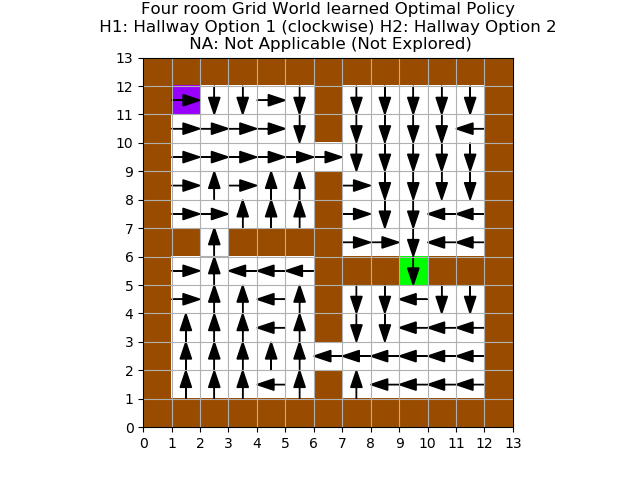
\includegraphics[width=0.4\linewidth]{./O1_10000_Arrows.png}\label{grid_a_arrow}}
	\subfigure[Grid world with goal G2]
	{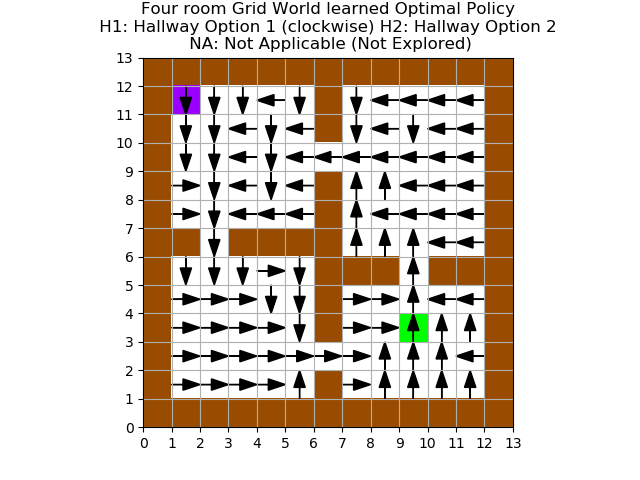
\includegraphics[width=0.4\linewidth]{./O2_10000_Arrows.png}\label{grid_b_arrow}}
	\caption{Grid world of four rooms.  Blue:Agent, Green:Terminal The grid world-\ref{grid_a_arrow} has terminal state G1 and grid world-\ref{grid_b_arrow} has terminal state G2. Arrow indicates the optimal policy. The policy in fig-\ref{grid_a_arrow} is obtained using option-1 where as same in fig.-\ref{grid_b_arrow} by option-2 }
	\label{fig:grids}
\end{figure}

For one move, agent is rewarded with 0. For terminal state reward is +1. With $\Pr = \frac{2}{3}$, the agent take correct action and other actions are performed with $\Pr = \frac{1}{9}$. The vale of discounted factor is $\gamma=0.9$. Each hallway option has termination condition 0 for states lies within room and 1 if outside. The initiation of state includes room as well as hallway. The initiation state is defined only inside the room which makes the world deterministic. To take agent from one room to another, there are two possible options. Option-1 follows the clockwise notation which take agent from room-1 to room-2. Option-2 follows anti-clockwise direction which can take agent from room-1 to room-4.

To solve the defined problem, SMDP and Intra-option Q learning is utilized. The optimal policy is the fundamental thing for used methods. To obtain the optimal policy using Q-learning, the initial states were randomly selected and goal is directed to hallway. likewise, eight policy is obtained. The state values are obtained using the maximum return.

\begin{equation}
	V(s) = \argmax_{Q(s,a)} 
\end{equation}

The obtained optimal policy for goal-G1 and G2 is given in fig.-\ref{fig:grids}. The visualization of state values are given in fig.-\ref{fig:state_val}. For goal both goals, higher state values are obtained near hallways and terminal state. High state values are indicated by bigger size of circle. 

\begin{figure}[H]
	\centering  
	\subfigure[State values with goal G1 by option-1]
	{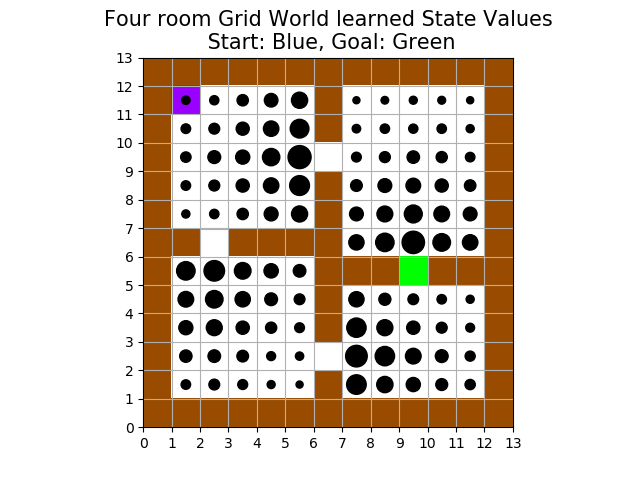
\includegraphics[width=0.4\linewidth]{./O1_10000_Circles.png}\label{grid_a_circle}}
	\subfigure[State values with goal G2 by option-2]
	{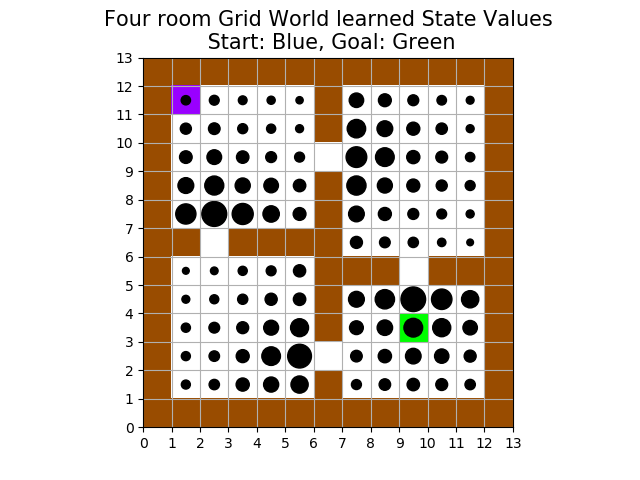
\includegraphics[width=0.4\linewidth]{./O2_10000_Circles.png}\label{grid_b_circle}}
	\caption{The grid world-\ref{grid_a_circle} has terminal state G1 and grid world-\ref{grid_b_circle} has terminal state G2. Circle size indicates the associated state value. The values in fig-\ref{grid_a_circle} is obtained using option-1 where as same in fig.-\ref{grid_b_circle} by option-2}
	\label{fig:state_val}
\end{figure}

\textbf{SMDP Q-learning :}

Semi Markov Decision Processes are generalized MDPs, which allows policy maker to choose action according to change in state. It also provides the evolution of policy with continuous time while following arbitrary probability distribution. In short, SMDP follows the similar nature of MDP with options. Execution option starts with state $\mathcal{I}$ following policy $\pi$ and jumps to terminating state s'. The SMDP Q-learning updates for option-value function is given by,
\begin{equation}
	Q(s,o)  = Q(s,o) + \alpha [ r + \gamma^k \max_{o'\in s'} Q(s',o') - Q(s,o)]
\end{equation}
where, \\
k -  the number of time steps between s' and s \\
r - Cummulative discounted return over time\\

\newpage 

\textbf{For Goal-G1:}

The learned optimal policy by SMDP-Q learning for goal-G1 is given in fig.-\ref{SMDP_G1_policy}. \textbf{The optimal policy is resultant of defined policy and primitive actions as well.} The primitive action are better than option away from goal and near the start state. Whereas, \textbf{near the terminal state Q-values are high and options play crucial role.}

Same can be observed from the state value diagram. \textbf{Near the goal state has higher valuer, which decrease as we move away from the goal.} Due to property of learning from experience and bound of wall near terminal state, in near the goal region there might be high chances of stumbling.  Some of the states are not explored as it possible to reach toward goal by following any option from those states. 

\begin{figure}[H]
	\centering  
	\subfigure[Optimal policy by SMDP-Q]
	{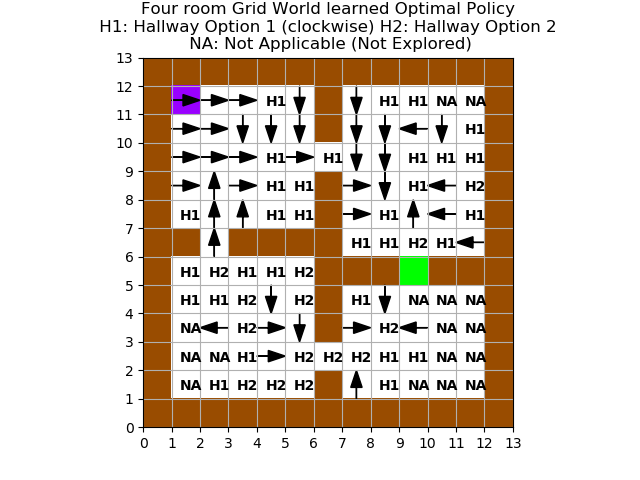
\includegraphics[width=0.39\linewidth]{./Q1_G1_10000_Arrows.png}\label{SMDP_G1_policy}}
	\subfigure[State values for SMDP-Q]
	{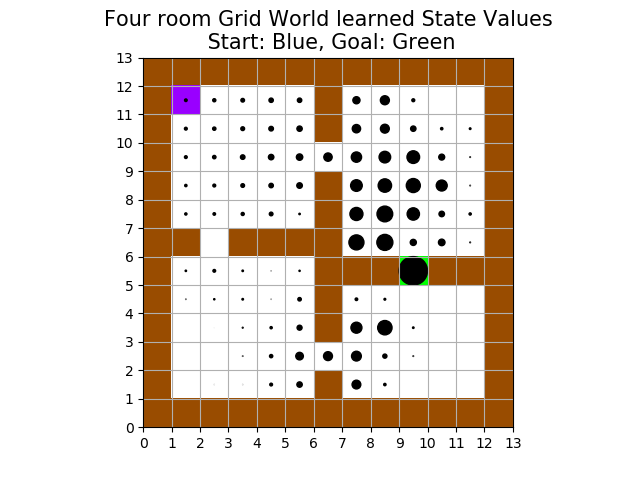
\includegraphics[width=0.39\linewidth]{./Q1_G1_10000_Circles.png}\label{SMDP_G1_value}}
	\caption{Grid world of four rooms.  Blue:Agent, Green:Terminal. The optimal policy-\ref{SMDP_G1_policy} and associated state values-\ref{SMDP_G1_value} for Goal-G1 after training of 10000 episodes.}
	\label{fig:SMDP_G1}
\end{figure}

\textbf{For Goal-G2:}

The optimal policy for goal-G2 is given in fig.\ref{SMDP_G2_policy}. For this case also, states near the goal selects primitive action over policy as it helps agent to move away from the hallways and direct it towards goal whereas, states away from the goal follows actions. From figure-\ref{fig:SMDP_G2}, it is clear that SMDP Q-learning has obtained optimal policy using \textbf{mix of primitive action as well as options.}

\begin{figure}[H]
	\centering  
	\subfigure[Optimal policy by SMDP-Q]
	{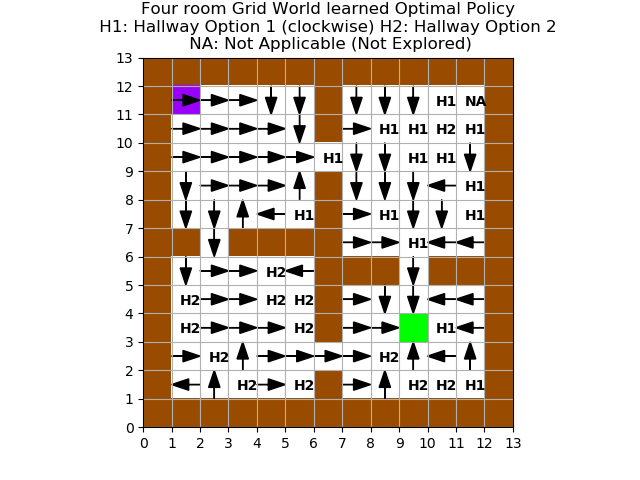
\includegraphics[width=0.39\linewidth]{./Q1_G2_10000_Arrows.png}\label{SMDP_G2_policy}}
	\subfigure[State values for SMDP-Q]
	{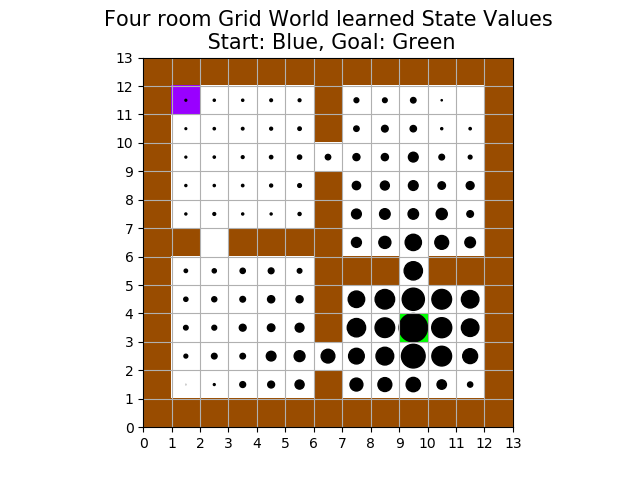
\includegraphics[width=0.39\linewidth]{./Q1_G2_10000_Circles.png}\label{SMDP_G2_value}}
	\caption{Grid world of four rooms.  Blue:Agent, Green:Terminal. The optimal policy-\ref{SMDP_G2_policy} and associated state values-\ref{SMDP_G2_value} for Goal-G2 after training of 10000 episodes.}
	\label{fig:SMDP_G2}
\end{figure}

 For goal-2 compared to goal-1, the major states follow primitive actions where as options are dominant in case of goal-G1. Mainly for room-1 policy plays major role, whereas for room 2 and 4 it requires both.  \textbf{Near terminal state, dominance of policy make algorithm faster by increasing the learning rate.}


\subsection{Answers-2 : Changed initial state to the centre of room 4}

For the same terminal state, initial state is directed to center of room-4. \textbf{The change in state also causes the change in value function and optimal policy.} The optimal policy obtained in these cases are also mixtures of options as well as primitive actions. 

\begin{figure}[H]
	\centering  
	\subfigure[Optimal policy by SMDP-Q for goal G1]
	{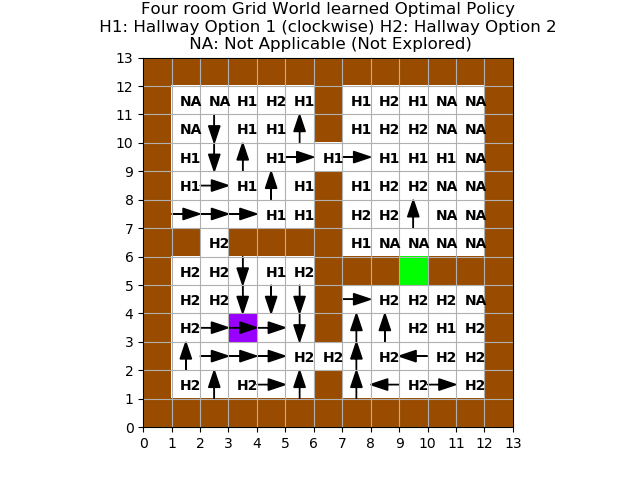
\includegraphics[width=0.39\linewidth]{./Q2_G1_10000_Arrows.png}\label{R4_SMDP_G1_policy}}
	\subfigure[State values for SMDP-Q for goal G1]
	{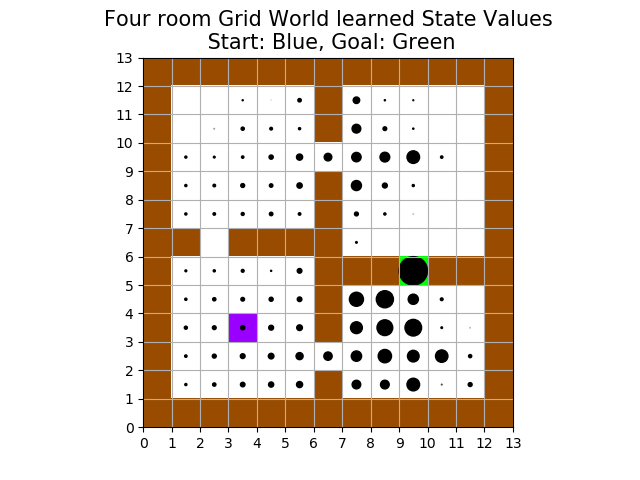
\includegraphics[width=0.39\linewidth]{./Q2_G1_10000_Circles.png}\label{R4_SMDP_G1_value}}
	\subfigure[Optimal policy by SMDP-Q for goal G2]
	{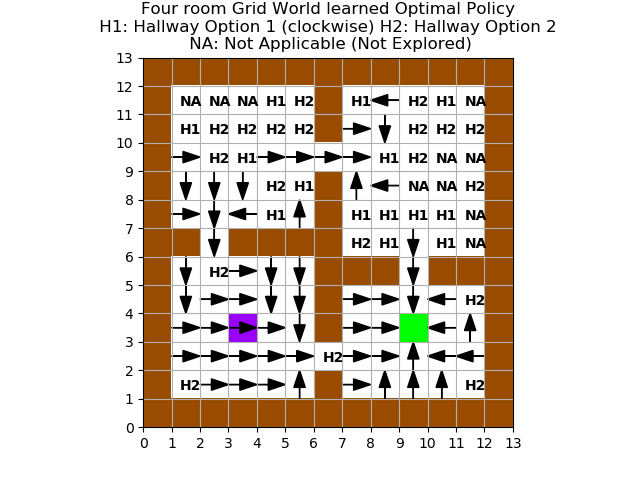
\includegraphics[width=0.39\linewidth]{./Q2_G2_10000_Arrows.png}\label{R4_SMDP_G2_policy}}
	\subfigure[State values for SMDP-Q for goal G2]
	{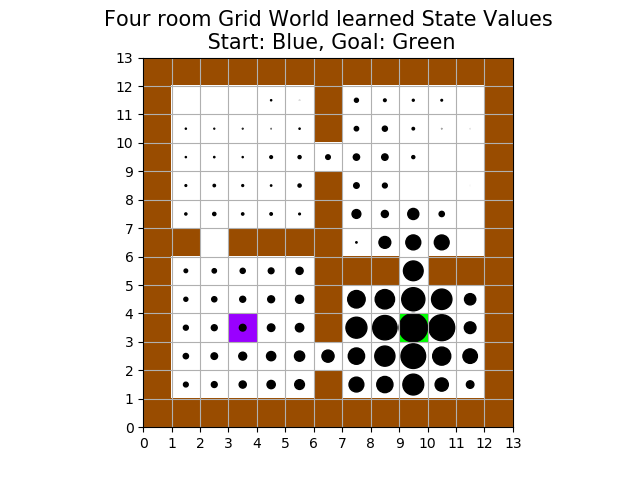
\includegraphics[width=0.39\linewidth]{./Q2_G2_10000_Circles.png}\label{R4_SMDP_G2_value}}
	\caption{Grid world of four rooms.  Blue:Agent, Green:Terminal. The optimal policy-\ref{R4_SMDP_G1_policy} and associated state values-\ref{R4_SMDP_G1_value} for Goal-G1 after training of 10000 episodes. Same way, the optimal policy-\ref{R4_SMDP_G2_policy} and associated state values-\ref{R4_SMDP_G2_value} for Goal-G2}
	\label{fig:R4_SMDP}
\end{figure}

Change of state does not affect the role of primitive action and policy near the terminal states as well as far away from it. The major difference in both scenario (policy for same goal and change of initial state) is change in state value function. By comparing the fig.-\ref{SMDP_G1_policy} and fig.-\ref{R4_SMDP_G1_policy}, it is clear that the \textbf{state value of adjutant room of terminal and start state has higher state values. Change of the initial state directly affect the optimal policy, which varies in both scenario and finds the best possible route using primitive action and options.}

 The value obtained in case of goal G2 is higher and shows nature of gradient. As goal-G1 is constrained by two wall these varies in this case. Options play vital role near terminal state of goal-G1, whereas, primitive actions play important role in case of goal-G2.

\subsection{Answers-3: Intra-option Q learning}

\section{Deep Reinforcement Learning:}
 For contentious state and action space. policy gradient algorithm are implemented. \cite{david}

	
\subsection{Answers-1: Hyper-parameter Tuning}	
\subsection{Answers-2: Report of hyper-parameters tuning}
\subsection{Answers-3: Report of the variation of hyper-parameters like hidden layer sizes, epsilon, mini-batch size, target frequency.}  
\subsection{Answers-4: Observations and inferences of removal of the experience replay and/or the target network}

	\newpage
	
	References:
	\\
	
	%%
	%% Following citation commands can be used in the body text:
	%% Usage of \cite is as follows:
	
	%%   \cite{key}          ==>>  [#]
	%%   \cite[chap. 2]{key} ==>>  [#, chap. 2]
	%%   \citet{key}         ==>>  Author [#]
	
	%% References with bibTeX database:
	\bibliographystyle{ieeetr}
	\bibliography{biblio.bib}					
	%% Authors are advised to submit their bibtex database files. They are
	%% requested to list a bibtex style file in the manuscript if they do
	%% not want to use model1-num-names.bst.
	
	%% References without bibTeX database:
	
	% \begin{thebibliography}{00}
	
	%% \bibitem must have the following form:
	%%   \bibitem{key}...
	%%
	
	% \bibitem{}
	
	% \end{thebibliography}


\end{document}